
São funções do tipo: $f: \mathbb{R}^3 \longrightarrow \mathbb{R}$.

Superfícies de nível são um conjunto de pontos no espaço tridimensional onde uma função de três variáveis atinge um valor constante. Elas são obtidas ao igualar a função a uma constante, como $f(x,y,z) = k$. Essa visualização tridimensional é análoga às curvas de nível usadas em mapas topográficos para representar a altitude.

\medskip
\begin{figure}[ht]
  \centering
  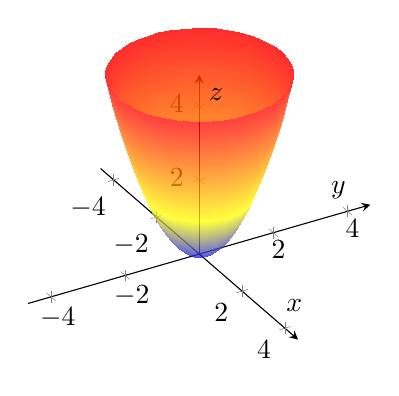
\begin{tikzpicture}
    \begin{axis}[
      view={60}{30},
      axis lines=middle,
      xlabel={$x$}, ylabel={$y$}, zlabel={$z$},
      domain=0:360,          % theta em graus
      y domain=0:2.2,        % r (raio)
      samples=50,            % reduzido levemente para compilação mais rápida
      samples y=20,
      z buffer=sort,
      grid=major,
      axis equal,
    ]

      % 1) "Sino" (paraboloide) com domínio circular
      \addplot3[
        surf,
        shader=interp,
        opacity=0.75,
        draw=none
      ]
      (
        {y*cos(x)},           % x = r cos(theta)
        {y*sin(x)},           % y = r sin(theta)
        {y^2}                 % z = r^2
      );

      % 2) "Boca plana": disco no topo z = R^2
      \addplot3[
        surf,
        shader=interp,
        opacity=0.30,
        draw=none
      ]
      (
        {y*cos(x)},
        {y*sin(x)},
        { (2.2)^2 }
      );

    \end{axis}
  \end{tikzpicture}
  \caption{parabolóide}
\end{figure}

\begin{enumerate}
  \item \textbf{Equação do Plano:}
  \[
    z = ax + by + c
  \]
  \[
    \Big\{ (x,y,z)\in \mathrm{Dom}(f)\ \big|\ f(x,y,z)=k \Big\}
  \]

  \item \textbf{Paraboloide Elíptico.} Para $a, b > 0$:
  \[
    z = ax^2 + by^2
  \]

  \item \textbf{Paraboloide Hiperbólico.}
  \[
    z = ax^2 - by^2
  \]

  \item \textbf{Cilindros.}
  \begin{enumerate}
    \item \textbf{Cilindro Parabólico.} Cada corte $y=c$ é uma parábola.
    \[
      z = x^2
    \]
    \item \textbf{Cilindro Elíptico.}
    \[
      x^2 + y^2 = 1
    \]
  \end{enumerate}

  \item \textbf{Superfícies Quádricas.}
  \begin{enumerate}
    \item \textbf{Elipsoide.}
    \[
      \frac{x^2}{a^2} + \frac{y^2}{b^2} + \frac{z^2}{c^2} = 1
    \]
    \item \textbf{Hiperboloide de uma folha.}
    \[
      \frac{x^2}{a^2} + \frac{y^2}{b^2} - \frac{z^2}{c^2} = 1
    \]
    \item \textbf{Hiperboloide de duas folhas.}
    \[
      -\frac{x^2}{a^2} - \frac{y^2}{b^2} + \frac{z^2}{c^2} = 1
    \]
  \end{enumerate}

  \bigskip
  \begin{table}[H]
    \centering
    \caption{Sinais dos coeficientes das superfícies quádricas usuais}
    \label{tab:quadricas}
    \begin{tabular}{lccc}
      \toprule
      \textbf{Superfície} & \textbf{a} & \textbf{b} & \textbf{c} \\
      \midrule
      Elipsoide             & + & + & + \\
      Hiperboloide 1 folha  & + & + & - \\
      Hiperboloide 2 folhas & - & - & + \\
      \bottomrule
    \end{tabular}
  \end{table}

  \item \textbf{Superfícies Esféricas.}
  A esfera não é uma função de $(x,y)$.

  \item \textbf{Superfícies Compostas.}
  \begin{enumerate}
    \item \textbf{Cone.}
    \[
      z = \sqrt{x^2+y^2}
    \]
    \item \textbf{Superfície Helicoidal.}
    \[
      \begin{cases}
        x = r \cos(\theta) \\
        y = r \sin(\theta) \\
        z = c\,\theta
      \end{cases}
    \]
    onde: $r$ é o raio; $\theta$ é o parâmetro angular (rad); $c$ controla o passo da hélice.
  \end{enumerate}
\end{enumerate}

Para funções de uma variável $y=f(x)$, temos:
\[
  \lim_{x \to x_0} f(x)
\]

\textbf{Exemplo.}
\[
  f(x,y,z) = x^2 + y^2 + z^2
\]
Domínio: $D(f)=\mathbb{R}^3$ e Imagem: $I(f)=[0,\infty)$.

As \textbf{superfícies de nível} são dadas por:
\[
  x^2 + y^2 + z^2 = c
\]
\begin{itemize}
  \item Se $c>0$: esfera de centro $(0,0,0)$ e raio $\sqrt{c}$.
  \item Se $c=0$: reduz-se ao ponto $(0,0,0)$.
  \item Se $c<0$: não existe superfície de nível (conjunto vazio).
\end{itemize}

\textbf{Exemplo.}
Seja a equação $z^2 - 3(x^2 + y^2) = 0$.
Isolando os termos:
\[
  \frac{z^2}{3} = x^2 + y^2
\]
Isso representa um \textbf{cone circular duplo}.

\begin{figure}[H]
  \centering
  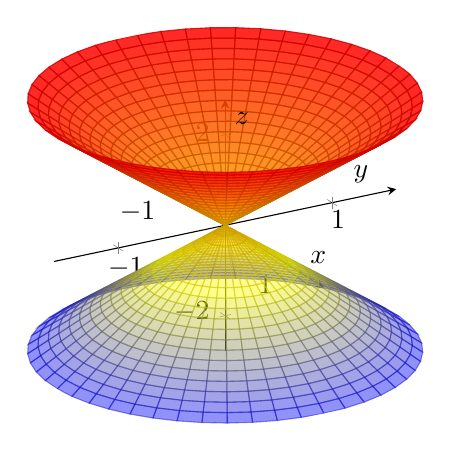
\begin{tikzpicture}
    \begin{axis}[
      view={60}{30},
      axis lines=middle,
      xlabel={$x$}, ylabel={$y$}, zlabel={$z$},
      domain=0:360, y domain=0:1.6,
      samples=50, samples y=20,
      z buffer=sort,
      grid=major,
    ]
      % Parametrização: x = r cos(theta), y = r sin(theta), z = ±sqrt(3) r
      \addplot3[surf, opacity=0.85, draw=none]
        ({y*cos(x)}, {y*sin(x)}, {sqrt(3)*y});
      \addplot3[surf, opacity=0.45, draw=none]
        ({y*cos(x)}, {y*sin(x)}, {-sqrt(3)*y});
    \end{axis}
  \end{tikzpicture}
  \caption{Cone circular duplo: $z^2 - 3(x^2+y^2)=0$.}
\end{figure}

Se $c=1$ na equação $\frac{z^2}{3} - x^2 - y^2 = c$, temos um \textbf{hiperboloide de duas folhas}. Se $c=-1$, o gráfico será um \textbf{hiperboloide de uma folha}.

